%%%%%%%%%%%%%%%%%%%%%%%%%%%%%%%%%%%%%%%%%
% University/School Laboratory Report
% LaTeX Template
% Version 3.1 (25/3/14)
%
% This template has been downloaded from:
% http://www.LaTeXTemplates.com
%
% Original author:
% Linux and Unix Users Group at Virginia Tech Wiki 
% (https://vtluug.org/wiki/Example_LaTeX_chem_lab_report)
%
% License:
% CC BY-NC-SA 3.0 (http://creativecommons.org/licenses/by-nc-sa/3.0/)
%
%%%%%%%%%%%%%%%%%%%%%%%%%%%%%%%%%%%%%%%%%

%----------------------------------------------------------------------------------------
%	PACKAGES AND DOCUMENT CONFIGURATIONS
%----------------------------------------------------------------------------------------

\documentclass{article}

\usepackage{graphicx} % Required for the inclusion of images
\usepackage{amsmath} % Required for some math elements
\usepackage{enumitem}
\usepackage{subcaption}

\setlength\parindent{0pt} % Removes all indentation from paragraphs

\renewcommand{\labelenumi}{\alph{enumi}.} % Make numbering in the enumerate environment by letter rather than number (e.g. section 6)

\newlist{inlinelist}{enumerate*}{1}
\setlist*[inlinelist,1]{%
  label=(\arabic*),
}

%----------------------------------------------------------------------------------------
%	DOCUMENT INFORMATION
%----------------------------------------------------------------------------------------

\title{\begin{LARGE}
	\textbf{EE 445L - Lab 3: Alarm Clock}
\end{LARGE}} % Title

\author{Joshua Bryant \\ jmb6357 \and James Morris \\ jsm3288} % Author name

\date{\today} % Date for the report

\begin{document}

\maketitle % Insert the title, author and date

%----------------------------------------------------------------------------------------
%	SECTION 1 Objectives
%----------------------------------------------------------------------------------------

\section{Objective}
	\subsection{Overview}
		\subsubsection{Objectives}
			The objectives of this project are to design, build and test a brushed DC motor controller. The motor should spin at a constant speed and the operator can specify the desired set point. Educationally, students are learning how to interface a DC motor, how to measure speed using input capture, and how to implement a digital controller running in the background.
		\subsubsection{Process}
			The project will be developed using the EK-TM4C123GXL or EK-TM4C1294XL LaunchPad. There will be two switches that the operator will use to specify  the desired speed of the motor. The system will be built on a solderless breadboard and run on the usual USB power. The system may use the on board switches or off-board switches. A hardware/software interface will be designed that allows software to control the DC motor. There will be at least five hardware/software modules: tachometer input, switch input, motor output, LCD output, and the motor controller. The process will be to design and test each module independently from the other modules. After each module is tested, the system will be built and tested.
		\subsubsection{Roles and Responsibilities}
			EE445L students are the engineers and the TA is the client. James Morris will build and test the sensor system. Joshua Bryant will build the actuator and switch input. Both students will work on the controller.
		\subsubsection{Interactions with Existing Systems}
			The system will use the microcontroller board, a solderless breadbaord, and the DC motor. The wiring connector for the DC motor is described in the PCB Artist file \textbf{Lab4B\_Artist.sch}. It will be powered using the USB cable. You may use a +5V power from the lab bench, but please do not power the motor with a voltage above +5V. 
		\subsubsection{Terminology}
			\begin{description}
				\item[Integral Controller]
					A controller whose output is proportional to the error of the output of the system compared to the desired setpoint.
				\item[Pulse Width Modulation (PWM)]
					A technique to deliver a variable signal (voltage, power, energy) using an on/off signal with a variable percentage of time the signal is on (duty cycle).
				\item[Board Support Package (BSP)]
					A set of software routines that abstract the I/O hardware such that the same high-level code can run on multiple computers.
				\item[Back EMF]
					A large voltage potential induced across an inductor due to large changes in current with respect to time ($\frac{dI}{dt}$) according to the equation $V=L*\frac{dI}{dt}$.
				\item[Torque]
					Available force times distance the stepper motor can provide at a given speed.
				\item[Time Constant]
					The time to reach 63.2\% of the final output after the input is instantaneously increased.
				\item[Hysteresis]
					A condition when the output of a system depends not only on the input, but also on the previous outputs, e.g., a transducer that follows a different response curve when the input is increasing than when the input is decreasing.
			\end{description}
		\subsubsection{Security}
			The system may include software from TivaWare and from the book. No software written for this project may be transmitted, viewed, or communicated with any other EE445L student past, present, or future (other than the lab partner of course). IT is the responsibility of the team to keep its EE445L lab solutions secure.
	\subsection{Function Description}
	
		\subsubsection{Functionality}
			If all buttons are released, then the motor should spin at a constant speed. If switch 1 is pressed and released, the desired speed should increase by 5 rps, up to a maximum of 40 rps. If switch 2 is pressed and released, the desired speed should decrease by 5 rps, down to a minimum of 0 rps.\\
			Both the desired and actual speed should be plotted on the color LCD as a function of time.
		\subsubsection{Scope}
			Phase 1 is the preparation; phase 2 is the demonstration; and phase 3 is the lab report. Details can be found in the lab manual.
		\subsection{Prototypes}
			A prototype system running on the EK-TM4C123GXL or EK-TM4C1294XL LaunchPad and solderless breadboard will be demonstrated. Progress will be judged by the preparation, demonstration, and lab report.
		\subsubsection{Performance}
			The system will be judged by three qualitative measures. First, the software modules must be easy to understand and well-organized. Second, the system must employ an integral controller running in the background. There should be a clear and obvious abstraction, separating the state estimator, user interface, the controller and the actuator output. Backward jumps in the ISR are not allowed. Third, all software will be judged according to style guidelines. Software must follow the style described in Section 3.3 of the book. There are three quantitative measures. First, the average speed error at a desired speed of 60 rps will be measured. The average error should be less than 5 rps. Second, the step response is the time it takes for the new speed to hit 60 rps after the set point is changed from 40 to 60 rps. Third, you will measure power supply current to run the system. There is no particular need to minimize controller error, step response, or system current in this system.
		\subsubsection{Usability}
			There will be two switch inputs. The tachometer will be used to measure motor speed. The DC motor will operate under no load conditions.
		\subsubsection{Safety}
			The motor current under no load will be less than 100 mA. However, under heavy friction this current could be 5 to 10 times higher. Therefore, please run the motors unloaded. Connecting or disconnecting wires on the protoboard while power is applied will damage the microcontroller. Operating the circuit without a snubber diode will also damage the microcontroller. 
	\subsection{Deliverables}
	
		\subsubsection{Reports}
			A lab report is due October 4th, 2014. This report includes the final requirements documents.
		\subsubsection{Audits}
			The preparation is due at the beginning of the lab period October 24th.
		\subsubsection{Outcomes}
			There are three deliverables: preparation, demonstration, and report.
 
%----------------------------------------------------------------------------------------
%	SECTION 2 Hardware Design
%----------------------------------------------------------------------------------------
\section{Hardware Design}
	\begin{figure}[h]
		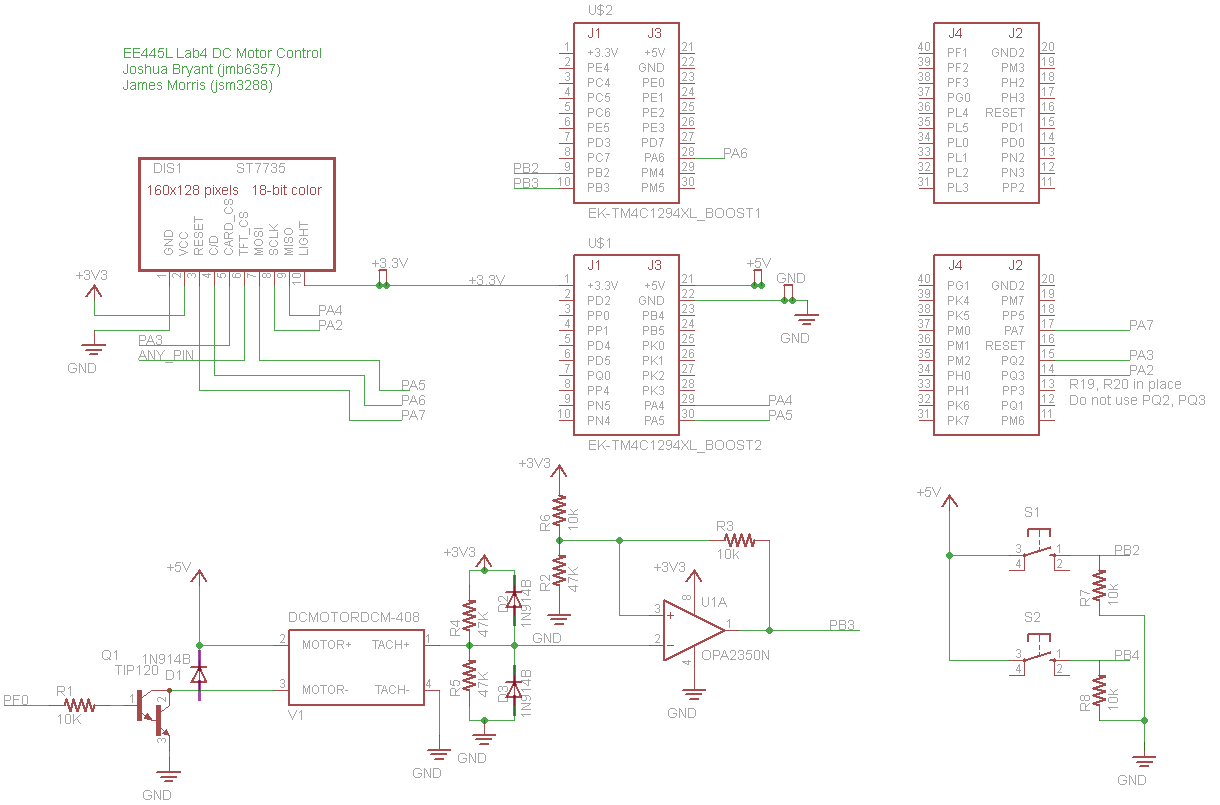
\includegraphics[keepaspectratio, width=\textwidth]{Lab4Graphics/finalSchematic.png}
	\end{figure}

%----------------------------------------------------------------------------------------
%	SECTION 3 Software Design
%----------------------------------------------------------------------------------------
%\section{Software Design}

%----------------------------------------------------------------------------------------
%	SECTION 4 Measurement Data
%----------------------------------------------------------------------------------------
\section{Measurement Data}
	\begin{enumerate}
		\item[1)]
			The resistance of the motor was measured to be 44.6 $\Omega$s. Below is the table of the measured current through and the voltage across the motor at no load. Please note that the motor did not spin until $\sim$2.5V was put across the motor.\\
			\begin{tabular}[h]{|c|c|}
				\hline
				Voltage (V) & Current (mA) \\	\hline
				1	&	0.3 \\	\hline
				2 	&	0.5	\\	\hline
				3	&	93	\\	\hline
				4	&	99	\\	\hline
				5	&	105	\\	\hline
			\end{tabular}
			
		\item[2)]
			The $I_{be}$ was $\sim$0.013 mA and the $I_{ce}$ was $\sim$85 mA.
			
		\item[3)]
			Below is the output signal of the tachometer after passing through the op-amp at two different running speeds of the motor.
			\centering		
			\begin{figure}[h]
				\centering
				\begin{subfigure}{0.45\textwidth}
					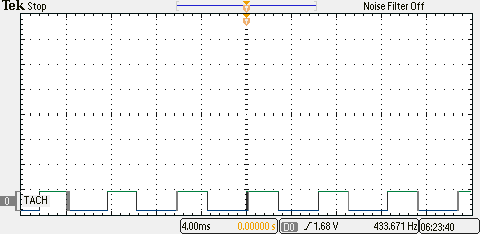
\includegraphics[keepaspectratio, width=\textwidth]{Lab4Graphics/TachMeasurement1}
					\caption{Tachometer Output at 50 rps}
					\label{fig:SS_TachMeasure1}
				\end{subfigure}
				\hfill
				\begin{subfigure}{0.45\textwidth}
					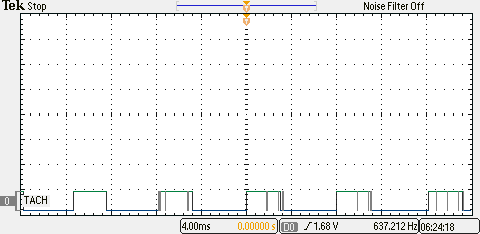
\includegraphics[keepaspectratio, width=\textwidth]{Lab4Graphics/TachMeasurement2}	
					\caption{Tachometer Output at 30 rps}
					\label{fig:SS_TachMeasure2}
				\end{subfigure}
				\caption{Screen shots of the oscilloscope measuring the tachometer signal output by the op-amp at two different running speeds of the motor.}
				\label{fig:SS_B&C}			
				\hfill		
			\end{figure}
			\raggedright		

		\item[4)]
			The maximum time to execute one instance of the ISR is $\sim$1.5 $\mu$s. The average controller error was measured at 5.2\%. The response time of our system is $\sim$0.5 s.
			
		\item[5)]
			The current of the system with the motor spinning was 209 mA while the current required to run the system with the motor stationary was 137 mA.
	\end{enumerate}
%----------------------------------------------------------------------------------------
%	SECTION 5 Analysis and Discussion
%----------------------------------------------------------------------------------------
\section{Analysis and Discussion}
	\begin{enumerate}
		\item %Question 1
			Torque is the turning force on an object. It's units of measure are Newton meters, NM, in SI.
		\item %Question 2
			\begin{figure}[h]
				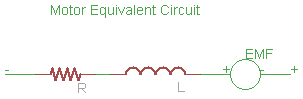
\includegraphics[keepaspectratio, width=\textwidth]{Lab4Graphics/motorCircuit.png}
			\end{figure}
			When the brushed DC-motor is allowed to free spin with no load, the back EMF (denoted by EMF) in the figure above, is nearly equivalent in magnitude and opposite in polarity to the voltage difference applied across the motor. The back EMF will be slightly less than the voltage differential causing a small voltage difference to form across the inductor and resistor allowing for a small, no-load current. When a load is applied, whether it be friction or another outside load, the back EMF produced by the motor drops in magnitude causing a larger voltage difference to form across the inductor and resistor leading to a higher current.
		\item %Question 3
			The important factors in selecting the motor drive interface chip were the Emitter-Base voltage, Collector-Emitter Voltage, and the total power dissipation. The max Collector-Emitter voltage for the TIP120 is 60V, the Emitter-Base voltage if 5V, and the total power dissipation is limited to 65W. Our circuit falls well within these requirements since the motor only requires a 6-20V difference to operate, we drive the base to 5V through the on-board power regulator of the TM4C1294 board, and the highest current measured through the motor was 209 mA leading to a maximum power dissipation being well under the maximum limit of the TIP120.
		\item %Question 4
			Instead of implementing only an integral controller, we could have implemented a full PID control loop. Or, if we got really fancy and knew more of the mechanical parameters of our system, we could implement a PID loop with a feed forward term.\\
			The PID control with a feed forward term would be superior to our current I control by allowing a faster response time to changing set point values as well as reduce initial bouncing of the output signal when first reaching a new set point as well as maintaining a smaller running error when maintaining a given set point, provided the loop is tuned correctly.
		\item %Question 5
			Given a motor rotating at a constant rate, the electrical power of the motor in Watts, $W_m$, is simply the product of the voltage across the motor, $V_m$, and the current through the motor, $I_m$. The equation for this is simply $W_m = V_m * I_m$.\\
			Mechanical power is, simply stated, the rate at which work is done. The official SI unit of power is the Watt (W), though it is more common, in mechanical terms, to deal with power in units of horsepower (hp). The conversion between horsepower and Watts is $1 hp \approx 745.7 W$.\\
			Yes, mechanical and electrical power are related. Both are still measures of power, each is just a specific measures in terms of different aspects of systems. Electrical power is used to relate how the measure of power is related to the control circuitry and what limitations on the output power are applied by the circuitry. The measure of mechanical power of a system is how much power the mechanical aspect of the system will be using/providing and what limitations there are on power with regards to the operation and safety of the mechanical hardware. In this way, mechanical and electrical power must be considered simultaneously when designing electro-mechanical systems.
	\end{enumerate}


\end{document}